% DO NOT COMPILE THIS FILE DIRECTLY!
% This is included by the other .tex files.

\begin{frame}[t,plain]
\titlepage
\end{frame}

\begin{frame}
\frametitle{Indicators - Problem Statement}
    \begin{itemize}
        \item Various users and organisations can share data via MISP, multiple parties can be involved
        \begin{itemize}
            \item \textbf{Trust}, \textbf{data quality} and \textbf{time-to-live} issues
            \item Each user/organisation has \textbf{different use-cases} and interests
                \begin{itemize}
                    \item Conflicting interests such as operational security, attribution,... (depends on the user)
                \end{itemize}
        \end{itemize}
        \item[] $\rightarrow$ Can be partially solved with \textit{Taxonomies}
        \pause
        \vspace{0.5cm}
        \item Attributes can be shared in large quantities (more than 7.3 million on \texttt{MISPPRIV})
        \begin{itemize}
            \item Partial info about their \textbf{freshness} (\textit{sightings})
            \item Partial info about their \textbf{validity} (last update)
        \end{itemize}
        \item[] $\rightarrow$ Can be partially solved with our \textit{Decaying model}
    \end{itemize}
\end{frame}

\begin{frame}
    \frametitle{\textit{Sightings} - Refresher}
    \textit{Sightings} add temporal context to indicators.
    A user, script or an IDS can extend the information related to indicators by reporting back to MISP that
    an indicator has been \texttt{seen}, or that an indicator can be considered as a \texttt{false-positive}
    \vspace{0.5cm}
    \begin{itemize}
        \item \textit{Sightings} give more credibility/visibility to indicators
        \item This information can be used to {\bf prioritise and decay indicators}
    \end{itemize}
    \begin{center}
        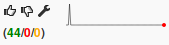
\includegraphics[scale=1.00]{pics/sightings.png}
    \end{center}
\end{frame}

\begin{frame}
\frametitle{Organisations opt-in - setting a level of confidence}
    MISP is a peer-to-peer system, information passes through multiple instances.
    \begin{itemize}
        \item Producers can add context (such as tags from \textit{taxonomies}, \textit{galaxies}) about their asserted confidence or the reliability of the data
        \item Consumers can have different levels of trust in the producers and/or analysts themselves
        \item Users might have other contextual needs
    \end{itemize}
\end{frame}

\begin{frame}
    \frametitle{Taxonomies - Refresher (1)}
    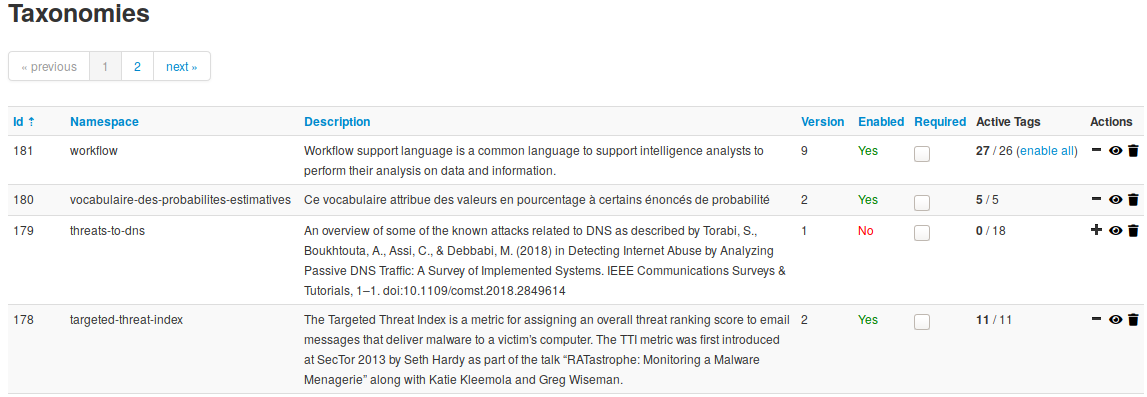
\includegraphics[width=1.00\linewidth]{pics/taxonomies.png}
\end{frame}

\begin{frame}
    \frametitle{Taxonomies - Refresher (2)}
    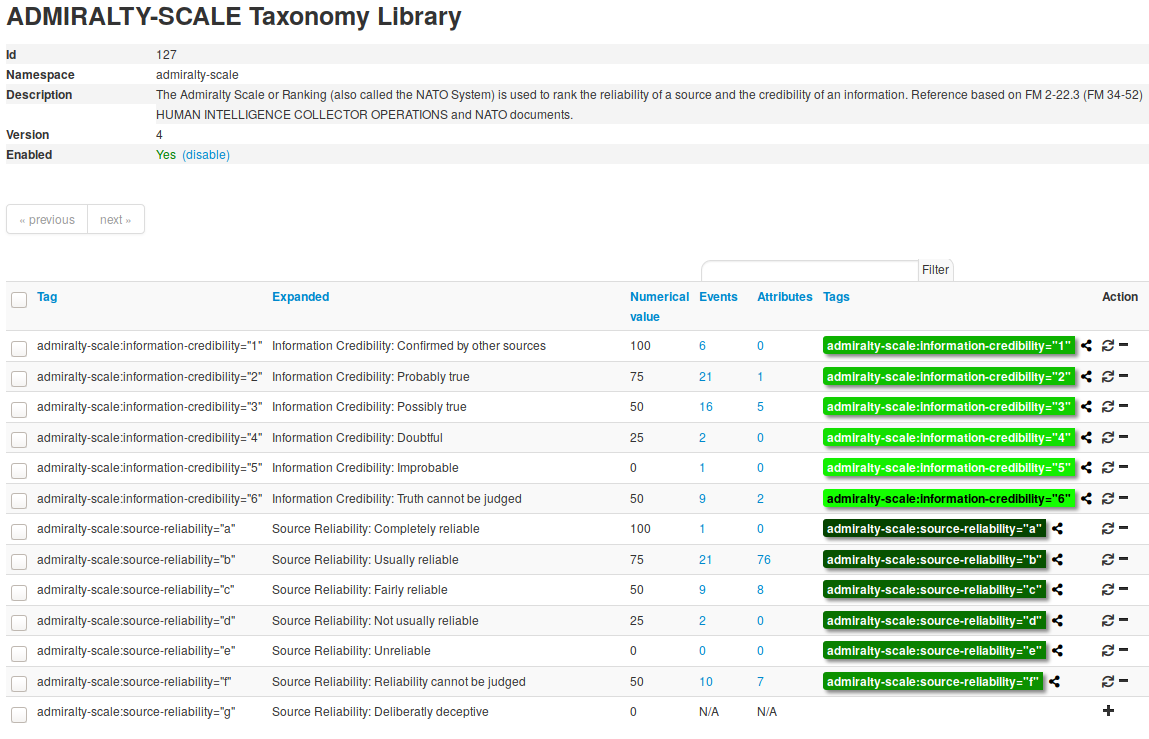
\includegraphics[width=1.00\linewidth]{pics/taxonomy-admiralty-scale.png}
\end{frame}

\begin{frame}
    \frametitle{Taxonomies - Refresher (3)}
    \begin{itemize}
        \item Some taxonomies have \texttt{numerical\_value}
        \begin{itemize}
            \item[$\rightarrow$] Can be used to prioritise \textit{Attributes}
        \end{itemize}
    \end{itemize}
    \vspace{1cm}

    \begin{footnotesize}
    \begin{columns}[T] % align columns
    \begin{column}{.40\textwidth}
        \begin{tabular}{|ll|}
            \hline
            \textbf{Description} & \textbf{Value}\\
            \hline
            Completely reliable & 100\\
            Usually reliable & 75\\
            Fairly reliable & 50\\
            Not usually reliable & 25\\
            Unreliable & 0\\
            Reliability cannot be judged & 50 \textbf{\color{red}?}\\
            Deliberatly deceptive & 0 \textbf{\color{red}?}\\
            \hline
        \end{tabular}
    \end{column}%
    \hfill%
    \begin{column}{.48\textwidth}
        \begin{tabular}{|ll|}
            \hline
            \textbf{Description} & \textbf{Value}\\
            \hline
            Confirmed by other sources & 100\\
            Probably true & 75\\
            Possibly true & 50\\
            Doubtful & 25\\
            Improbable & 0\\
            Truth cannot be judged & 50 \textbf{\color{red}?}\\
            \hline
        \end{tabular}
    \end{column}%
    \end{columns}
    \end{footnotesize}
\end{frame}

\begin{frame}
    \frametitle{Scoring Indicators: Our solution}
    $$ \texttt{score}(\texttt{\tiny Attribute}) = \texttt{base\_score}(\texttt{\tiny Attribute, Model}) \;\;\bullet\;\; \texttt{decay}(\texttt{\tiny Model, time}) $$
    Where,\vspace{0.5cm}
    \begin{itemize}
        \item \texttt{score} $ \in [0, +\infty $
        \item \texttt{base\_score} $ \in [0, 100] $
        \item \texttt{decay} is a function defined by model's parameters controlling decay speed
    \end{itemize}
    
\end{frame}

\begin{frame}
    \frametitle{Implementation in MISP: \texttt{Event/view}}
    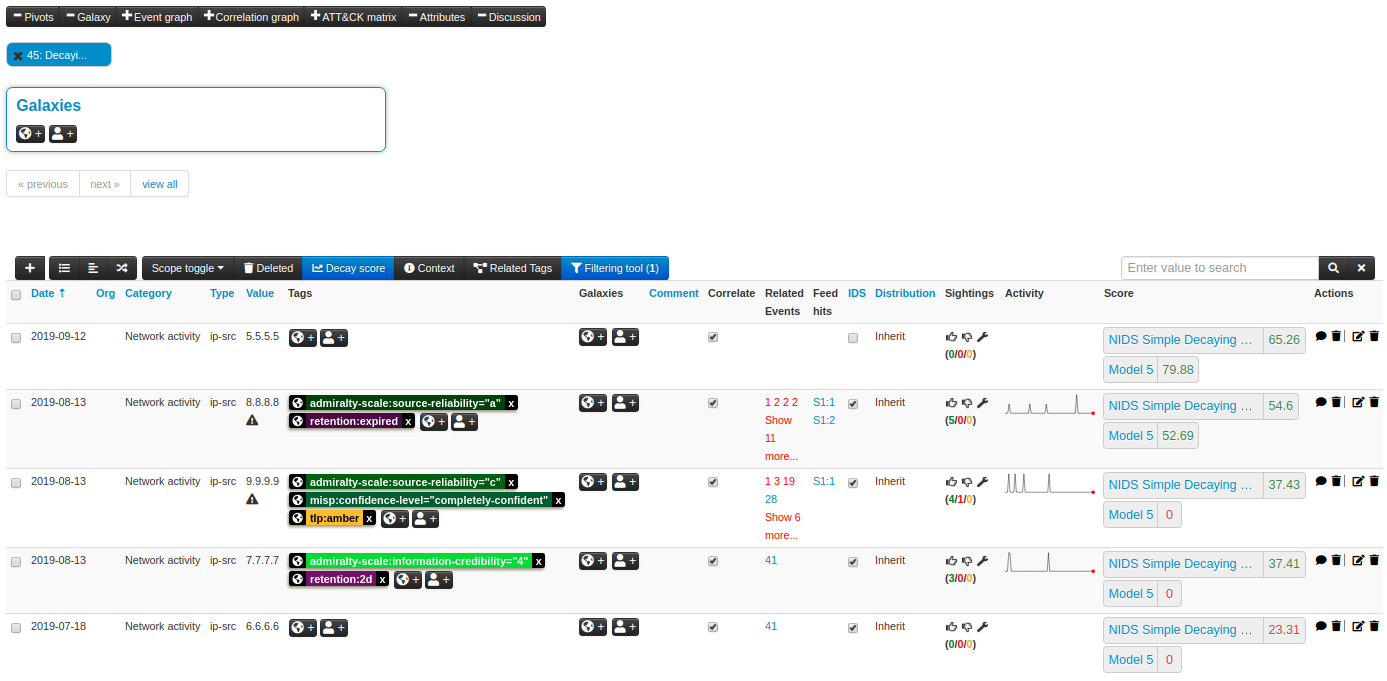
\includegraphics[width=1.00\linewidth]{pics/decaying-event.png}
\end{frame}

\begin{frame}[fragile]
    \frametitle{Implementation in MISP: API result}
    \texttt{/attributes/restSearch}
    \begin{lstlisting}
"Attribute": [
  {
    "category": "Network activity",
    "type": "ip-src",
    "to_ids": true,
    "timestamp": "1565703507",
    [...]
    "value": "8.8.8.8",
    "decay_score": [
      {
        "score": 54.475223849544456,
        "decayed": false,
        "DecayingModel": {
          "id": "85",
          "name": "NIDS Simple Decaying Model"
        }
      }
    ],
[...]
    \end{lstlisting}
\end{frame}

\begin{frame}
\frametitle{Implementation in MISP: Playing with Models}
    \begin{itemize}
        \item \textbf{Automatic scoring} based on default values
        \item \textbf{User-friendly UI} to manually set lifetime and decay parameters
        \item \textbf{Simulation} tool
        \item Interaction through the \textbf{API}
        \item Opportunity to create your \textbf{own} formula or algorythm
    \end{itemize}
\end{frame}

\begin{frame}
    \frametitle{Scoring Indicators: \texttt{base\_score} (1)}
    $$ \texttt{score}(\texttt{\tiny Attribute}) = \texttt{base\_score}(\texttt{\tiny Attribute, Model}) \;\;\bullet\;\; {\color{gray}\texttt{decay}(\texttt{\tiny Model, time})} $$
        When scoring indicators\footnote{Paper available: \url{https://arxiv.org/pdf/1803.11052}}, multiple parameters\footnote{at a variable extent as required} can be taken into account. The {\bf base score} is calculated with the following in mind:
    \begin{itemize}
        \item {\color{purple}Data reliability, credibility, analyst skills, custom prioritisation tags (economical-impact), etc.}
        \item {\color{orange}Trust in the source}
    \end{itemize}
    \vspace{0.3cm}
    $$\texttt{base\_score} = \omega_{tg} \cdot {\color{purple}tags} + \omega_{sc} \cdot {\color{orange}source\_confidence}$$
    Where,
    \begin{itemize}
        \item[] $\omega_{sc} + \omega_{tg} = 1$
    \end{itemize}
\end{frame}

\begin{frame}
    \frametitle{Scoring Indicators: \texttt{base\_score} (2)}
    Current implentation ignore \texttt{source\_confidence}:
    $$\rightarrow \texttt{base\_score} = tags$$
    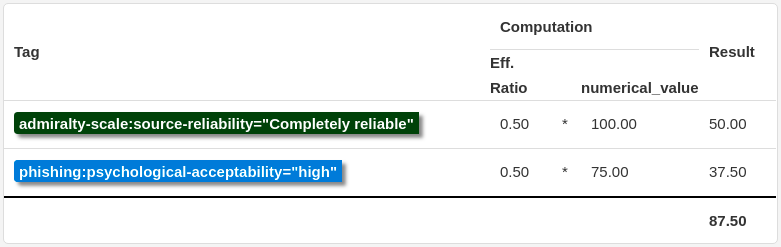
\includegraphics[width=1.0\linewidth]{pics/bs-computation-steps.png}
\end{frame}

\begin{frame}
    \frametitle{Scoring Indicators: decay speed (1)}
    $$ \texttt{score}(\texttt{\tiny Attribute}) = {\color{gray}\texttt{base\_score}(\texttt{\tiny Attribute, Model})} \;\;\bullet\;\; \texttt{decay}(\texttt{\tiny Model, time}) $$
    The \texttt{decay} is calculated using:
   \begin{itemize}
       \item The \texttt{lifetime} of the indicator
       \begin{itemize}
           \item May vary depending on the indicator type
           \item short for an IP, long for an hash
       \end{itemize}
       \item The \texttt{decay rate}, or speed at which an attribute loses value over time
       \item The time elapsed since the latest update or sighting
   \end{itemize}
\end{frame}

\begin{frame}
    \frametitle{Scoring Indicators: putting it all toghether}
    $\rightarrow$ \texttt{decay rate} is \textbf{re-initialized upon sighting} addition, or said differently, the \texttt{score} is reset to its base score as new \textit{sightings} are applied.
    $$score = base\_score \cdot \left( 1 - \left( \frac{t}{\tau_a} \right)^{\frac{1}{\delta_a}} \right) $$
    \begin{itemize}
        \item $\tau_a = $ \texttt{lifetime}
        \item $\delta_a = $ \texttt{decay speed}
    \end{itemize}
\end{frame}

\begin{frame}
    \frametitle{Implementation in MISP: Models definition}
    \textit{Models} are an instanciation of the formula where elements can be defined:
    \begin{itemize}
        \item Parameters: \texttt{lifetime, decay\_rate, threshold}
        \item \texttt{base\_score}
        \item \texttt{default base\_score}
        \item formula
        \item associate \textit{Attribute} types
        \item creator organisation
    \end{itemize}
\end{frame}

\begin{frame}
    \frametitle{Implementation in MISP: Models Types}
    Multiple model types are available
    \begin{itemize}
        \item Default models: Models created and shared by the community. Available from \texttt{misp-decaying-models} repository\footnote{\url{https://github.com/MISP/misp-decaying-models.git}}.
        \begin{itemize}
            \item $\rightarrow$ Not editable
        \end{itemize}
        \item Organisation models: Models created by a user belonging to an organisation
        \begin{itemize}
            \item These models can be hidden or shared to other organisation 
            \item $\rightarrow$ Editable
        \end{itemize}
    \end{itemize}
\end{frame}

\begin{frame}
    \frametitle{Implementation in MISP: Index}
    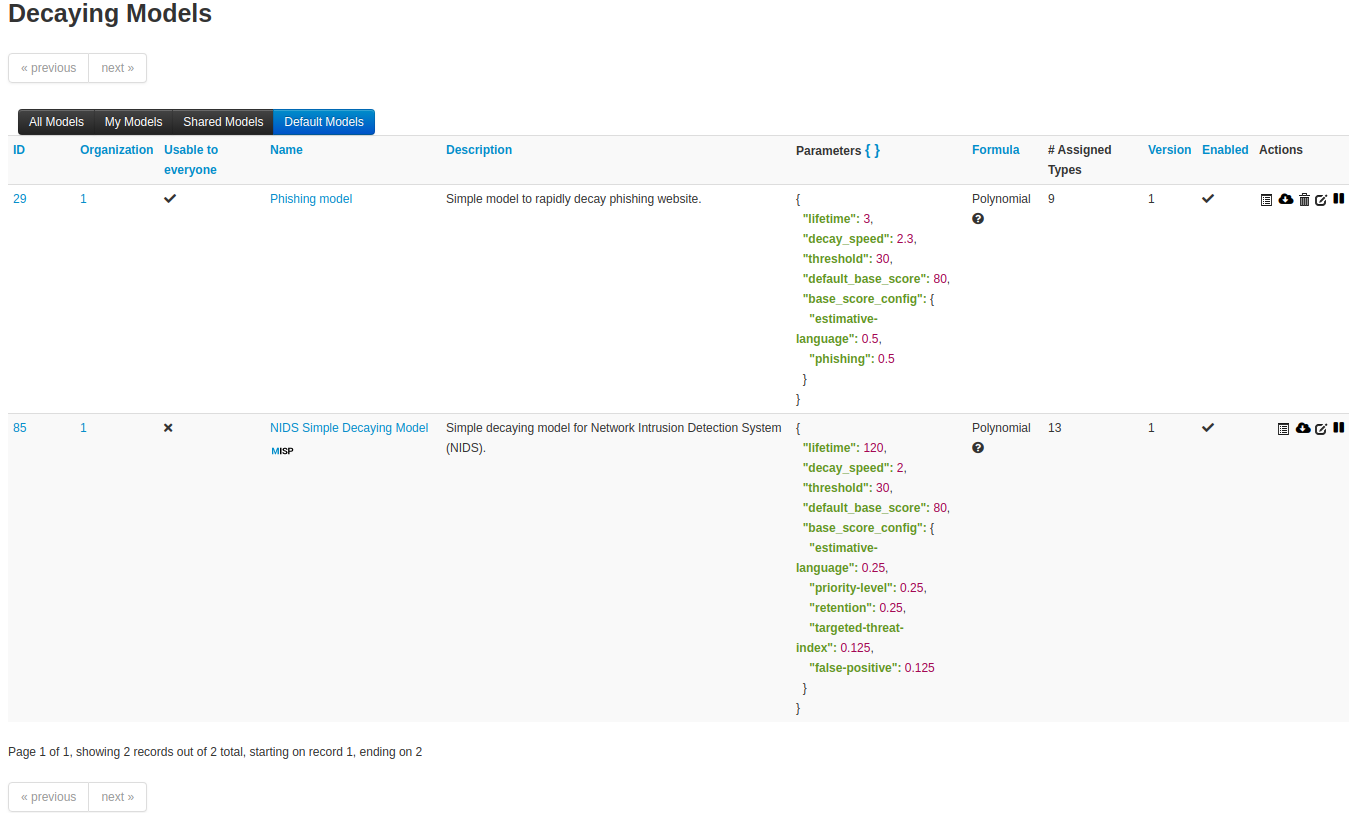
\includegraphics[width=1.00\linewidth]{pics/decaying-index.png}
\end{frame}

\begin{frame}
    \frametitle{Implementation in MISP: Fine tuning tool}
    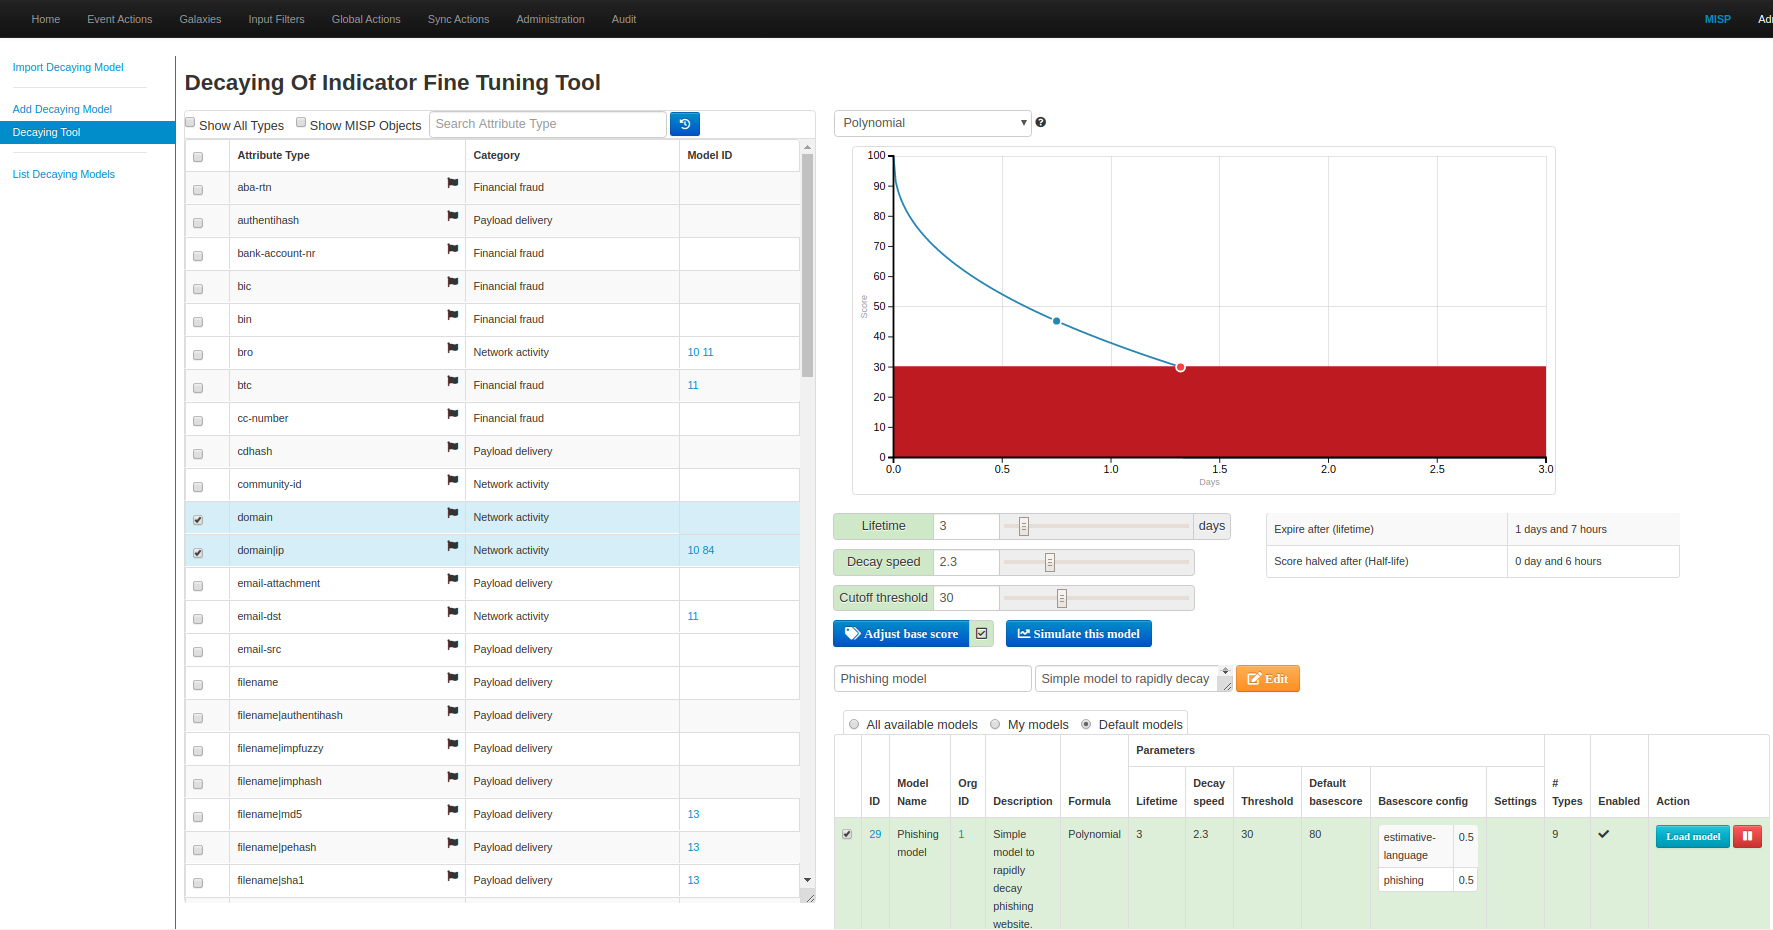
\includegraphics[width=1.00\linewidth]{pics/decaying-tool.png}
\end{frame}

\begin{frame}
    \frametitle{Implementation in MISP: \texttt{base\_score} tool}
    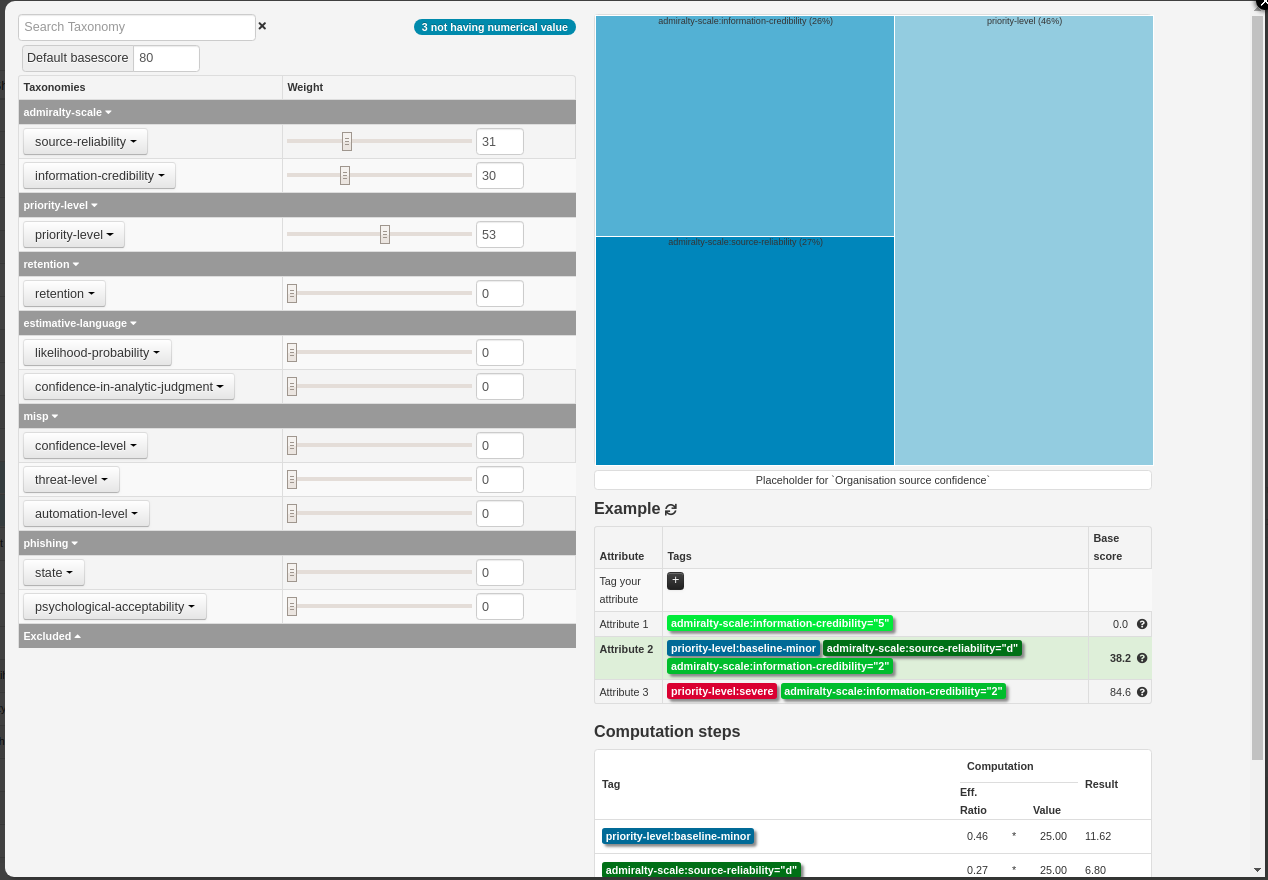
\includegraphics[width=1.00\linewidth]{pics/decaying-basescore.png}
\end{frame}

\begin{frame}
    \frametitle{Implementation in MISP: simulation tool}
    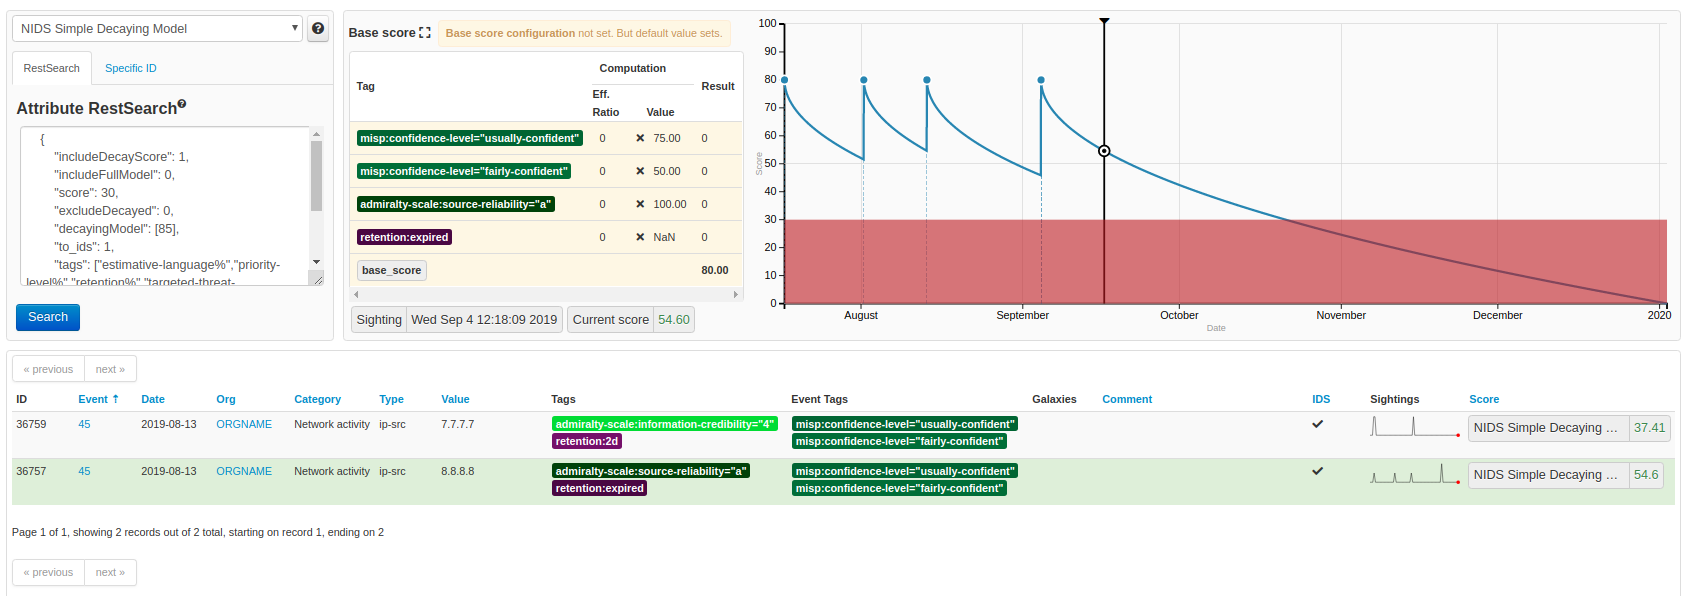
\includegraphics[width=1.00\linewidth]{pics/decaying-simulation.png}
\end{frame}

\begin{frame}[fragile]
    \frametitle{Implementation in MISP: API query body}
    \texttt{/attributes/restSearch}
    \begin{lstlisting}
{
    "includeDecayScore": 1,
    "includeFullModel": 0,
    "excludeDecayed": 0,
    "decayingModel": [85],
    "modelOverrides": {
        "threshold": 30
    }
    "score": 30,
}
    \end{lstlisting}
\end{frame}

\begin{frame}
    \frametitle{Creating a new decay algorithm (1)}
    The current architecture allows users to create their \textbf{own} formulae.

    \begin{itemize}
        \item Create a new file \texttt{{\$}filename} in \texttt{app/Model/DecayingModelsFormulas/}
        \item Extend the Base class as defined in \texttt{DecayingModelBase}
        \item Implement the two mandatory functions \texttt{computeScore} and \texttt{isDecayed} using your own formula/algorithm
        \item Create a Model and set the formula field to \texttt{{\$}filename}
    \end{itemize}

    Use cases:
    \begin{itemize}
        \item Add support for \textbf{more feature} (expiration taxonomy)
        \item \textbf{Query external services} then influence the score
        \item Completely \textbf{different approach} (i.e streaming algorithm)
        \item ...
    \end{itemize}

\end{frame}

\lstset{language=PHP}
\begin{frame}[fragile]
    \frametitle{Creating a new decay algorithm (2)}
    \lstset{basicstyle=\scriptsize}
    \begin{lstlisting}
<?php
include_once 'Base.php';

class Polynomial extends DecayingModelBase
{
    public const DESCRIPTION = 'The description of your new decaying algorithm';

    public function computeScore($model, $attribute, $base_score, $elapsed_time)
    {
       // algorithm returning a numerical score
    }

    public function isDecayed($model, $attribute, $score)
    {
        // algorithm returning a boolean stating
        // if the attribute is expired or not
    }
}
?>
    \end{lstlisting}
\end{frame}
